\documentclass[letterpaper,12pt]{article}

% Packages
\usepackage{fixltx2e}
\usepackage[margin=2.54cm]{geometry}
\usepackage{amsmath}
\usepackage{amsfonts}
\usepackage{amsthm}
\usepackage{paralist}
\usepackage{float}
\usepackage{graphicx}
\usepackage{algorithmic}
\usepackage{tikz}
\usepackage{mathpartir}
\usetikzlibrary{positioning,shadows,arrows}
\usepackage{listings}
\usepackage{caption}

\lstset{
        basicstyle=\footnotesize\ttfamily,
        numbers=left,
        numberstyle=\tiny,
        breaklines=true
        keywordstyle=\color{red},
        stringstyle=\color{white}\ttfamily,
        frame=b,
        showspaces=false,
        showtabs=false,
        xleftmargin=17pt,
        framexleftmargin=17pt,
        framexrightmargin=5pt,
        framexbottommargin=4pt,
        showstringspaces=false
}

\lstloadlanguages{
        Java
}

\DeclareCaptionFont{white}{\color{white}}
\DeclareCaptionFormat{listing}{
        \colorbox[cmyk]{0.43, 0.35, 0.35,0.01}{
                \parbox{\textwidth}{\hspace{15pt}#1#2#3}
        }
}

\captionsetup[lstlisting]{
        format=listing,
        labelfont=white,
        textfont=white,
        singlelinecheck=false,
        margin=0pt,
        font={bf,footnotesize}
}

\begin{document}

\title{Assignment 1}
\date{February 24, 2012}
\author{CPSC 433 \\ David Z. Chen}

\maketitle

\section{Asynchronous Server}

The architecture of the asynchronous server \texttt{SHTTPAsyncServer} closely follows that of the Asynchronous Server V3. A new \texttt{ReadWriteHander} (\texttt{SHTTPReadWriteHandler}) was implemented to handle HTTP requests. The request handling code was based heavily on the handler code used by the synchronous servers, \texttt{WebRequestHander}, but adapted for asynchronous socket I/O. Another change made was that the load balancing callback is now made to the \texttt{Dispatcher} object rather than the instance of the \texttt{SHTTPAsyncServer}.

In order to implement timeout, a separate thread that monitors timeout events of different opened sockets is instantiated along with the Dispatcher thread. When the Acceptor handler accepts a connection, after creating the \texttt{ReadWriteHandler}, it registers a timeout event for the \texttt{ReadWriteHandler}'s selection key. The selection key is added to the \texttt{IdleTimer}'s asynchronous queue, which is processed at the beginning of each iteration of the timeout thread's run loop. Later, when the \texttt{ReadWriteHandler} completes reading the request, it sends a cancellation request to the timeout thread, which is placed in another asynchronous queue in the timeout thread.

The timeout thread should not close the channel directly because the Dispatcher will still have the key registered and will not be able to know about the closing of the channel so that it may deregister the key. The timeout thread maintains two asynchronous queues and a \texttt{HashMap} that tracks the end-times of timeout events that are keyed by their selection key. The main loop of the timeout thread is as follows. First, it checks its timeout registration queue and adds each selection key to the HashMap with the end-time set to the current time plus the incomplete timeout set by the server's configuration file. Then, it checks its cancellation request queue and removes each of the requested timeout events from the HashMap. 

Finally, it iterates through all of the timeout events in the HashMap. For each key-value pair found, it checks whether the current time has passed the end-time. If it has, then a new \texttt{IdleTimerTask} object is created, which is a simple Runnable whose \texttt{run()} method simply calls the method of the Dispatcher to close the channel associated with a particular selection key. The Dispatcher was modified to also contain an asynchronous queue based on \texttt{invokeLater()} from Santos's article. The timer thread adds the task to the Dispatcher's asynchronous queue using \texttt{invokeLater()}, and the Dispatcher closes the channel associated with that selection key and deregisters the key.


\section{Comparison of Designs}

Reflecting our discussion in class, asynchronous servers are extremely complex. The xsocket library is a hybrid architecture, both asynchronous and multi-threaded. With the significant gain in performance, also comes a significant gain in complexity and difficulty of tracing execution paths through the server.

\subsection{Dispatcher threads}

According to the xsocket documentation, by default, xsocket creates $\text{number of CPUs} + 1$ dispatcher threads. The dispatcher threads, represented by the \texttt{IoSocketDispatcher} class, are managed in a \texttt{IoSocketDispatcherPool}.

The dispatchers are created as follows. First, a \texttt{Server} object is created. The \texttt{Server} constructor calls \texttt{ConnectionUtils.getIoProvider().createAcceptor()} on line 489. The \texttt{createAcceptor()} method of \texttt{IoProvider} (IoProvider.java line 471) instantiates a \texttt{IoAcceptor} object (IoProvider.java line 478). The \texttt{IoAcceptor} constructor instantiates a \texttt{IoSocketDispatcherPool} (IoAcceptor.java line 119), passing it a size, which \texttt{IoSocketDispatcherPool} uses when it calls \texttt{setDispatcherSize()} (IoSocketDispatcherPool.java line 77) to set the size of the dispatcher thread pool. After it sets the size, it calls \texttt{updateDispatcher()} on line 290. The first time this method is called, it notices that the number of dispatcher threads running is less than the maximum and instantiates each dispatcher thread (line 178). Before instantiating each dispatcher, it creates a \texttt{IoUnsynchronizedMemoryManager} object for the dispatcher (line 172-176).

The way that the dispatcher pool shares the workload may be seen in the \texttt{accept()} method of \texttt{IoAcceptor}. The \texttt{nextDispatcher()} method of \texttt{IoSocketDispatcherPool} allows the dispatcher threads to be retrieved and assigned in a round-robin fashion. After retrieving the next dispatcher thread, the acceptor simply assigns it the new connection.

\subsection{Workflow of dispatcher}

As described above, a dispatcher thread is represented by the \texttt{IoSocketDispatcher} class. Its constructor is defined in IoSocketDispatcher.java line 106-127. The constructor is passed a memory manager object and a string name. It then opens a \texttt{Selector}. \texttt{IoSocketDispatcher} is \texttt{Runnable}. The \texttt{run()} method of the dispatcher is as follows:

\begin{lstlisting}[label=dispatcherLoop,caption=Main loop of dispatcher,firstnumber=208]
    public void run() {
        
        // set thread name and attach dispatcher id to thread
        Thread.currentThread().setName(name);
        THREADBOUND_ID.set(id);

        DIRECT_CALL_COUNTER.set(0);

        if (LOG.isLoggable(Level.FINE)) {
            LOG.fine("selector " + name + " listening...");
        }

        int handledTasks = 0;

        while(isOpen.get()) {
            try {
                int eventCount = selector.select(5000);

                handledTasks = performRegisterHandlerTasks();
                handledTasks += performKeyUpdateTasks();

                if (eventCount > 0) {
                    handleReadWriteKeys();
                }

                handledTasks += performDeregisterHandlerTasks();

                checkForLoooping(eventCount + handledTasks, lastTimeWokeUp);

            } catch (Throwable e) {
                // eat and log exception
                if (LOG.isLoggable(Level.FINE)) {
                    LOG.fine("[" + Thread.currentThread().getName() + "] exception occurred while processing. Reason " + DataConverter.toString(e));
                }
            }
        }
        

        for (IoSocketHandler socketHandler : getRegistered()) {
            socketHandler.onDeregisterEvent();
        }

        try {
            selector.close();
        } catch (Exception e) {
            // eat and log exception
            if (LOG.isLoggable(Level.FINE)) {
                LOG.fine("error occured by close selector within tearDown " + DataConverter.toString(e));
            }
        }
    }
\end{lstlisting}

The main loop iterates as long as the Dispatcher is open. Each time through the loop, it calls \texttt{select()} (line 224). Then, it calls \texttt{performRegisterHandlerTasks()} (line 226) which runs all of the tasks on the asynchronous queue \texttt{registerQueue} to handle each of the register handler tasks. Then, it calls texttt{performKeyUpdateTasks()} (line 227) which similarly runs each task for updating selection keys on the asynchronous queue \texttt{keyUpdateQueue}. Then, if handlers have been registered and if selection keys have been updated, it means that there could be read and write events that need to be handled. Thus, it calls \texttt{handleReadWriteKeys()} which, similar to our dispatcher, loops through the set of selection keys and calls the read and write handlers for the read and write events. Then, it calls \texttt{performDeregisterHandlerTasks()} to run the tasks on the asynchronous queue \texttt{deregisterQueue} for deregistering handlers. Finally, it checks whether the thread is idle-looping by calling the parent class's \texttt{checkForLooping()} method, which has the thread either sleep or reinitialize the selector if idle looping is detected. Finally, if the dispatcher thread has closed, the loop terminates. Then, all of the \texttt{IoSocketHandler} objects are deregistered and the selector is closed.

\subsection{\texttt{EchoHandler} calling sequence}

\subsubsection{System Initialization}

The trace will begin with the initialization of the server. In EchoServerTest.java on line 50, a new \texttt{EchoServer} object is created with 0 as the listen port number. The constructor of \texttt{EchoServer} is defined on EchoServer.java line 54. In the constructor, a \texttt{EchoHandler} is first instatiated on line 56. Then, a new \texttt{Server} object is instantiated on line 68 and is passed the port number and the \texttt{EchoHandler}. The server's constructor (Server.java line 483) calls \texttt{setHandler()} (line 498) which creates a \texttt{HandlerAdapter} object that wraps the \texttt{EchoHandler} passed to it.

The server is then set to asynchronous flush mode for the connection (line 69) and is then started (line 71). After the server is started, the server's \texttt{run()} method is invoked (Server.java line 586). Here, the server records the startup time (line 593), creates a handler to be invoked when the server shuts down (line 595), registers it (line 599) and calls the acceptor's \texttt{listen()} method (line 603). 

The acceptor contains a reference to a \texttt{LifeCycleHandler} object. The acceptor's \texttt{listen()} method first calls the \texttt{onConnected()} method of the \texttt{LifeCycleHandler} (IoAcceptor.java line 205) which initializes the server's listener objects. Then, the acceptor calls \texttt{accept()} to enter its main loop (IoAcceptor.java line 206).

\subsubsection{Making the connection}

To trace the call sequence for a request, we start in the main loop of the acceptor in IoAcceptor.java lines 212-233. The acceptor's main loop iterates as long as the acceptor is open. It first calls \texttt{accept()} on the acceptor's \texttt{ServerSocketChannel}. Note that in the constructor of \texttt{IoAcceptor} on line 111, \texttt{serverChannel} is set to be blocking. As a result, this \texttt{accept()} call will block. Once a connection is established, the acceptor retrieves the next dispatcher thread from the dispatcher thread pool in a round-robin manner (line 219), creates a \texttt{IoChainableHandler} (line 220), which is passed the dispatcer and the socket channel. Following the \texttt{createIoHandler()}, we see that the type of \texttt{IoChainableHandler} is \texttt{IoSocketHandler} (IoProvider.java line 512). Finally, the acceptor calls the \texttt{onConnectionAccepted()} method of the \texttt{LifeCycleHandler}, passing it the \texttt{IoChainableHandler} (line 223) and increments the number of connections accepted.

The \texttt{LifeCycleHandler} checks to see if the maximum number of connections have been exceeded (Server.java line 1134). If not, it creates a \texttt{NonBLockingConnection} object to represent the connection and initializes the connection (lines 1170-1171) and sets the timeout values (more in next section). The \texttt{NonBlockingConnection} is also the \texttt{EchoHandler}.

The initialization of \texttt{NonBlockingConnection} is fairly complex. It creates a new \texttt{HandlerAdapter} to contain the \texttt{EchoHandler} (NonBlockingConnection.java line 722). On line 1191 of Server.java, the \texttt{init()} method of the \texttt{NonBlockingConnection} is called and is passed the \texttt{IoChainableHandler}. Tracing to NonBlockingConnection.java line 1042, we see that this overloaded method simply calls the other \texttt{init()} method, passing the \texttt{IoSocketHandler} and a \texttt{IoHandlerCallback} called \texttt{ioHandlerCallback}. Note that the \texttt{IoHandlerCallback} class, defined on line 2465, is actually a callback object for the \texttt{NonBlockingConnection} itself, and this will be important later.

This \texttt{init()} method of the \texttt{NonBlockingConnection} then calls the \texttt{init()} method of the handler (line 1049), pasing the \texttt{IoHandlerCallback} callback object for itself. Finally, we see that the handler registers itself with the dispatcher in read mode (IoSocketHandler.java line 142). When the dispatcher registers the handler, it registers the handler's channel with its selector. As described in the xsocket documentation, a connection is associated with the same dispatcher for its entire lifecycle. We now continue our trace of the execution in the dispatcher's main loop.

\subsubsection{Dispatcher}

The dispatcher calls \texttt{select()} on line 224 of IoSocketDispatcher.java. If it detects that new handlers have been registers or selection keys have been updated, it calls \texttt{handleReadWriteKeys()} on line 230 (IoSocketDispatcher.java). This method is defined on line 261. It loops through each selection key. For each selection key, it obtains the attached \texttt{IoSocketHandler} on line 272. We recall that in the \texttt{EchoServerTest}, a short string \texttt{"test\textbackslash r\textbackslash n"} is written to the server. 

Thus, at this point, the key is readable, and the dispatcher calls \texttt{onReadableEvent()} on line 278, which in turn calls the \texttt{onReadableEvent()} method of the handler on line 301. Then, on line 296 of IoSocketHandler.java, the handler in turn calls \texttt{onData()} of its reference to the \texttt{IoHandlerCallback} of the \texttt{NonBlockingConnection}. This method is defined on line 1208 of \texttt{NonBlockingConnection} and simply calls \texttt{appendDataToReadBuffer()} if the \texttt{ByteBuffer} pased to it is not null. The \texttt{appendDataToReadBuffer()} method is inherited from its parent class, \texttt{AbstractNonBlockingStream} and is defined on line 1484 of AbstractNonBlockingStream.java. Here, the \texttt{ByteBuffer} and size read are appended to a \texttt{readQueue} and \texttt{onPostAppend()} is called (lines 1485 and 1486), which checks if the read buffer is full and suspends the current I/O thread (not the dispatcher thread) if the read buffer is full. In short, the sequence of calls starting with the \texttt{onData()} call of the \texttt{IoHandlerCallback} handles the sequence of asynchronous reads until the entire request has been read.

Then, we return to the \texttt{IoSocketHandler} which then calls its \texttt{IoHandlerCallback}'s \texttt{onPostData()} method on line 297 of IoSocketHandler.java. This method simply calls the \texttt{onPostData()} method of \texttt{NonBlockingConnection}, which obtains the \texttt{HandlerAdapter} containing \texttt{EchoHandler} atomically and calls the \texttt{HandlerAdapter}'s \texttt{onData()} method (NonBlockingConnection.java line 1316). This method is defined on line 164 of HandlerAdapter.java. This method eventually calls \texttt{performOnData()}, which is defined on line 221. Finally, \texttt{performOnData()} calls \texttt{EchoHandler}'s \texttt{onData()} method. This completes our trace.

\subsection{Idle timeout}

The xsocket framework tests for two kinds of timeout: connection and idle timeout. Idle timeout occurs when no data is received for a certain amount of time defined by the idle timeout time whereas the connection timeout is the timeout time for the entire lifetime of the connection.

A client-server connection is represented by a \texttt{NonBlockingConnection} object. In the \texttt{init()} method of the inner class \texttt{Server.LifeCycleHandler} (Server.java line 1184), the \texttt{setIdleTimeoutMillis()} method (line 1194) and the \texttt{setConnectionTimeoutMillis()} methods (line 1195) of \texttt{NonBlockingConnection} are called to set the idle and connection timeout times. Both methods are methods of the \texttt{IConnection} interface, which is used to represent an end-to-end connection or session that contains the backing socket channel.

The \texttt{NonBlockingConnection} class also provides the method \texttt{checkIdleTimeout()} (line 1401) and \texttt{checkConnectionTimeout()} (line 1427) that check whether the an idle timeout or a connection timeout has occurred.

The actual timeout checking is done by a \texttt{WachdogTask}, a private inner class of \texttt{ConnectionManager} (ConnectionManager.java line 237). This class extends \texttt{TimerTask} and is scheduled to be run at regular time intervals by a timer. Every time the \texttt{WachdogTask} is run, it calls \texttt{check()} (defined ConnectionManger.java line 257) which iterates through each \texttt{NonBlockingConnection} and calls the two aforementioned timeout checking methods (lines 294 and 299) via \texttt{checkTimeout()} (line 291).

\subsection{Testing}

Testing for xsocket is usually by done by instantiating a server object and executing client side code that connects with the server through a local socket and having the client code assert certain expected output from the server. In the \texttt{EchoServerTest}, the test code creates a \texttt{EchoServer} object, opens a local socket to the server, writes to it, and asserts if the same message is echoed back. This is possible because the server runs in separate threads. The second test \texttt{testXSocketBothSide} similarly sends the server requests and tests whether the response received is as expected, but it executes that code in a separate thread that simulates the client.

A way to test our server with idle timeout would be similar to the way that the xsocket \texttt{TimeoutTest} performs testing. The \texttt{TimeoutTest} tests both idle and connection timeouts by setting a timeout on the server, opening a connection from the client, and then stalling for a certain amount of time that would cause the server to timeout. To test for a specific timeout event, such as an idle timeout and not a connection timeout, it sets the connection timeout to a $t_c$ and the idle timeout to a $t_i$ such that $t_c > t_i$, open a connection, and have the client send an imcomplete request and sleep for a time $t$ such that $t_i < t < t_c$ and then check that the idle timeout event was triggered but the connection timeout has not.

Since our server does not implement connection timeout, we can simply assume that as long as data is being received, the connection will remain open. Let our timeout time be $t$ seconds. With proper adjustments to our server code, our test program can instantiate a server, then open a socket to the server and simply sleep for $t + 1$ seconds then wake up and check that the server has timeout and closed the connection.

\section{Performance benchmarking}

A set of test files and request pattern files were generated with the scripts provided in gen.tar. The same request pattern was used for all of the servers. Each server was tested on a separate zoo machine, and the zoo Apache server was benchmarked per the instructions on the assignment page. The thread pool servers were each tested with a small thread pool of 4 threads and a large thread pool of 24 threads. Transactional throughput in files per second was recorded for each benchmark. The results of the benchmark were graphed and are shown in Figure 1.

\begin{figure}[t]
	\centering
	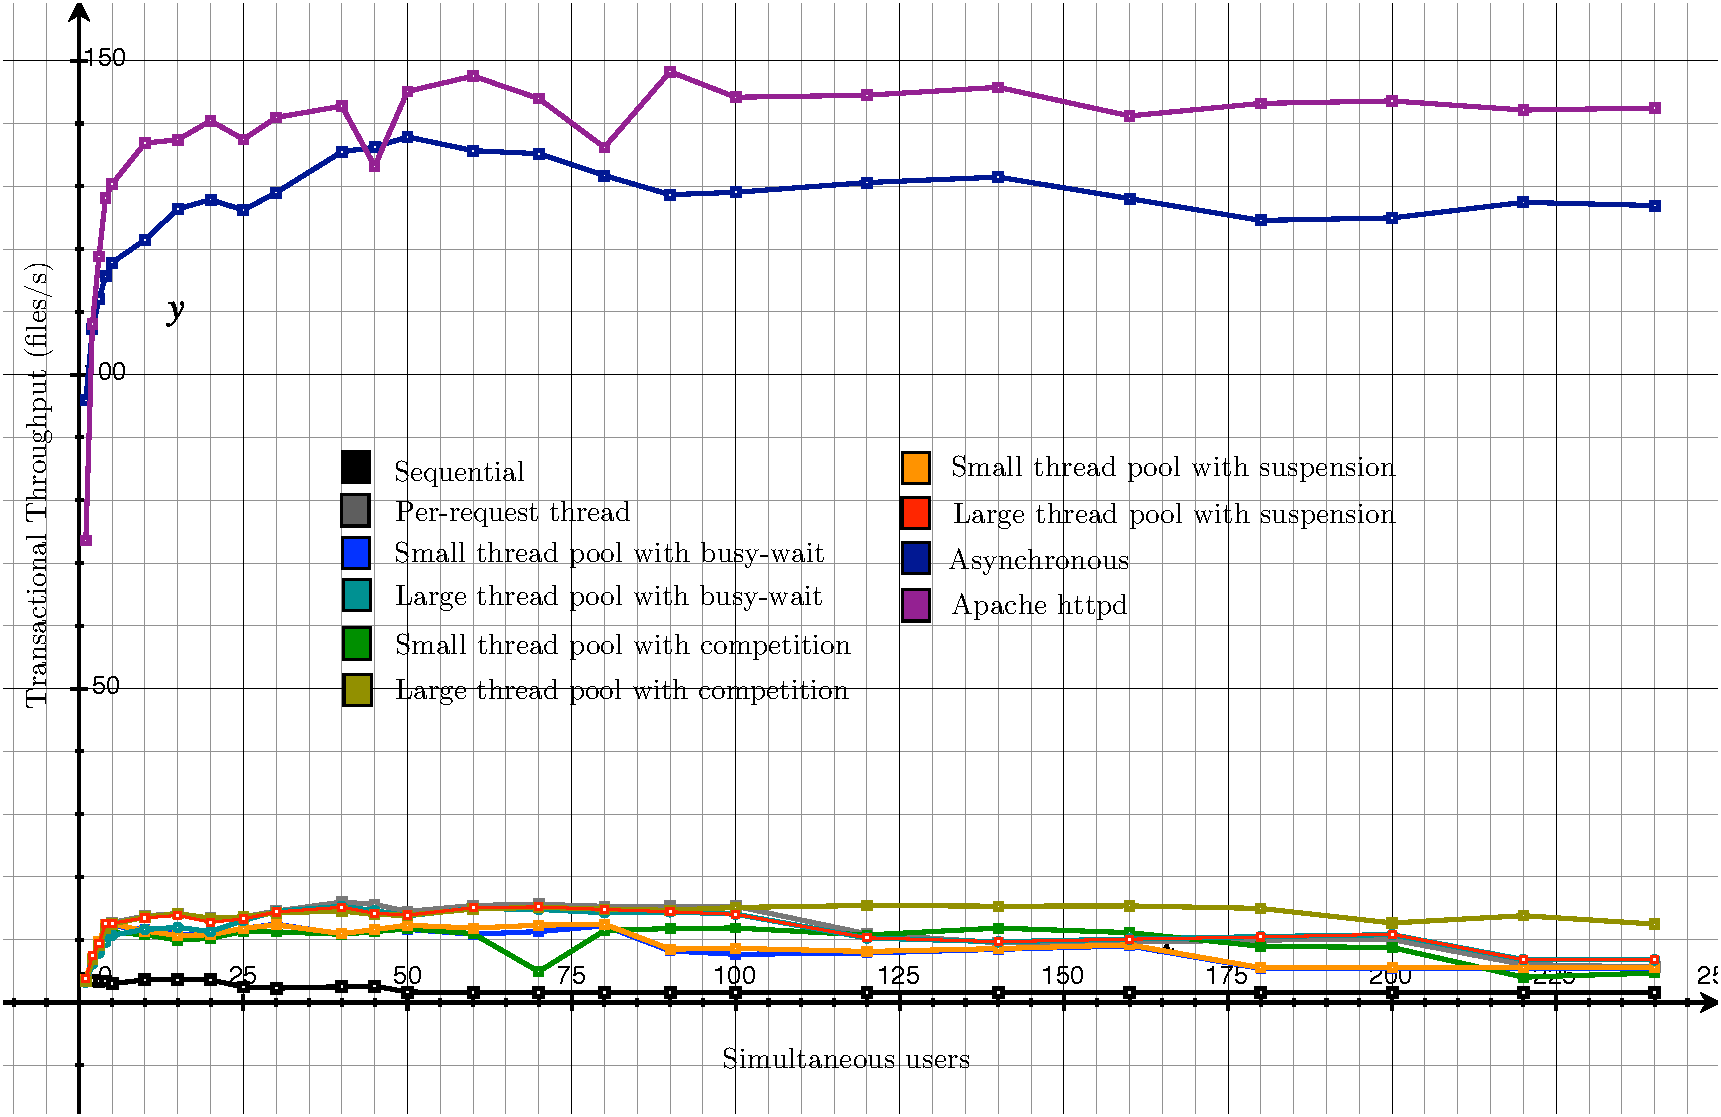
\includegraphics[width=1.0\textwidth]{doc/benchmarks_fig.pdf}
	\caption{Performance benchmarks with transactional throughput on the $y$ axis and number of simultaneous users (threads) on the $x$ axis.}
\end{figure}

As expected, the sequential server performs the worst. With a large number of simultaneous users, it becomes overwhelmed. The per-request server performs the best out of the threaded servers initially. However, at a certain point, the thread overhead begins to overtake the performance increase. 

Clearly, the asynchronous server greatly outperforms the sequential and all of the threaded servers by serveral orders of magnitude, though it is slightly outperformed by the more highly-optimized Apache. Although the event driven architecure is much more complex than the synchronous multithreaded ones, the improvement in performance is dramatic. 

\begin{figure}[t]
	\centering
	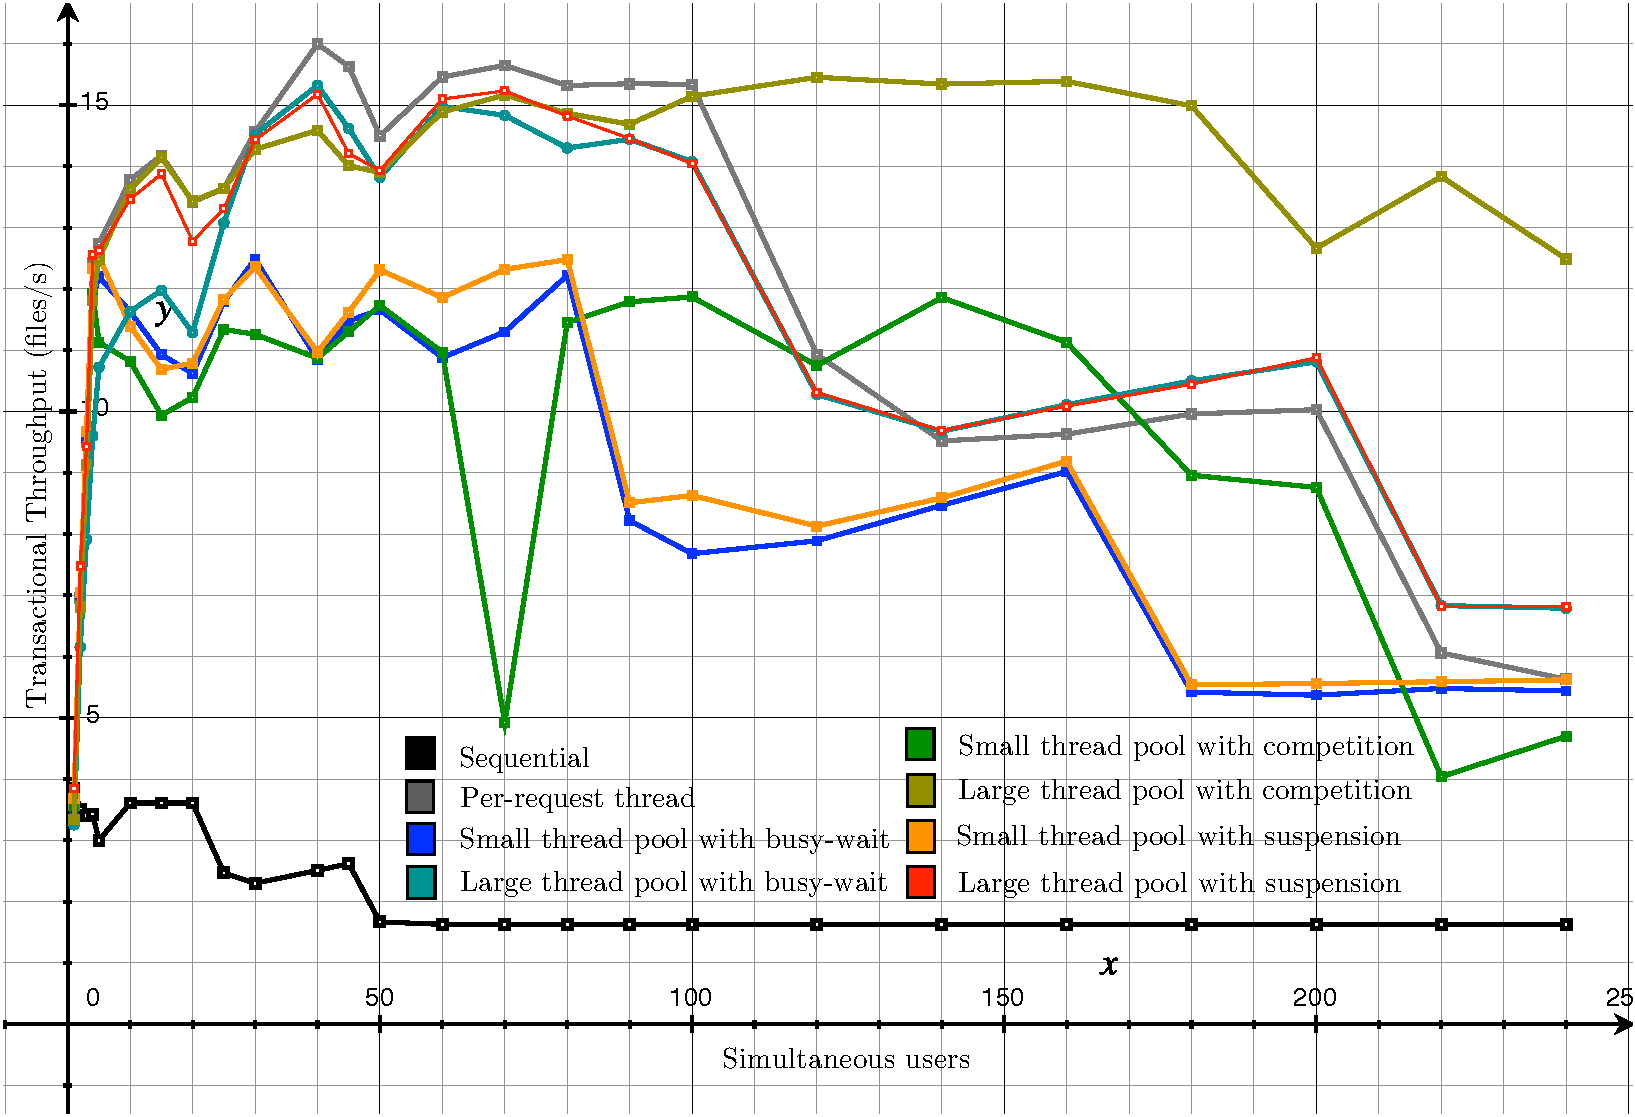
\includegraphics[width=1.0\textwidth]{doc/benchmarks_threaded_fig.pdf}
	\caption{Performance benchmarks in detail showing only the thread pool, per-request, and sequential servers.}
\end{figure}

For clarity, the graphs of the performance of threaded and sequential servers is shown in detail in Figure 2. For each of the thread pool servers, running with a large thread pool indeed increases throughput to a certain extent. However, this performance increase is nominal compared to the performance increase given by using asynchronous I/O. Furthermore, it is likely that at a certain point, the thread overhead will begin to overtake any performance advantage of a larger thread pool. 

\end{document}
